\documentclass[12pt, a4paper]{article}

\usepackage{array}
\usepackage[portuguese]{babel}
\usepackage{float}
\usepackage[a4paper, margin=2cm]{geometry}
\usepackage{graphicx}
\usepackage{hyperref}
\usepackage{setspace}
\usepackage{xcolor}

\title{\textbf{Computação Gráfica \\ \large Trabalho Prático -- Fase I}}
\date{2 de março 2025}
\author{Grupo \textbf{\color{red} TODO}}

\begin{document}

\begin{center}
    
\includegraphics[width=0.25\textwidth]{res/cover/EE-C.eps}
\end{center}

{\let\newpage\relax\maketitle}
\maketitle
\thispagestyle{empty}

\chardef\_=`_
\onehalfspacing
\setlength{\parskip}{\baselineskip}
\setlength{\parindent}{0pt}
\def\arraystretch{1.5}

\vspace{2cm}

\begin{center}
    \begin{tabular}{>{\centering}p{0.25\textwidth}
                    >{\centering\arraybackslash}p{0.25\textwidth}}
        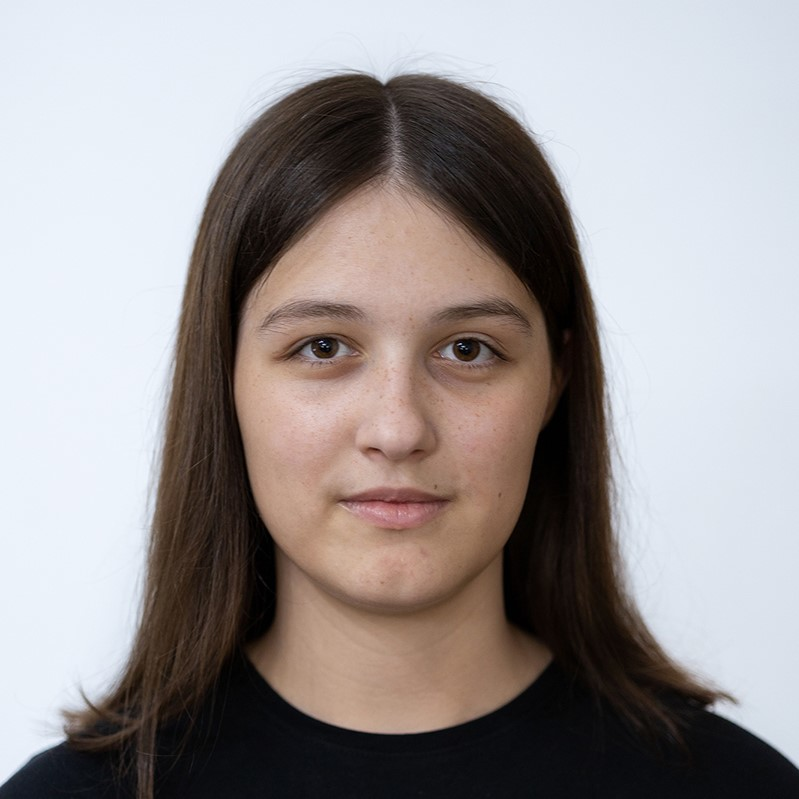
\includegraphics[width=3.5cm]{res/cover/A104437.png} &
        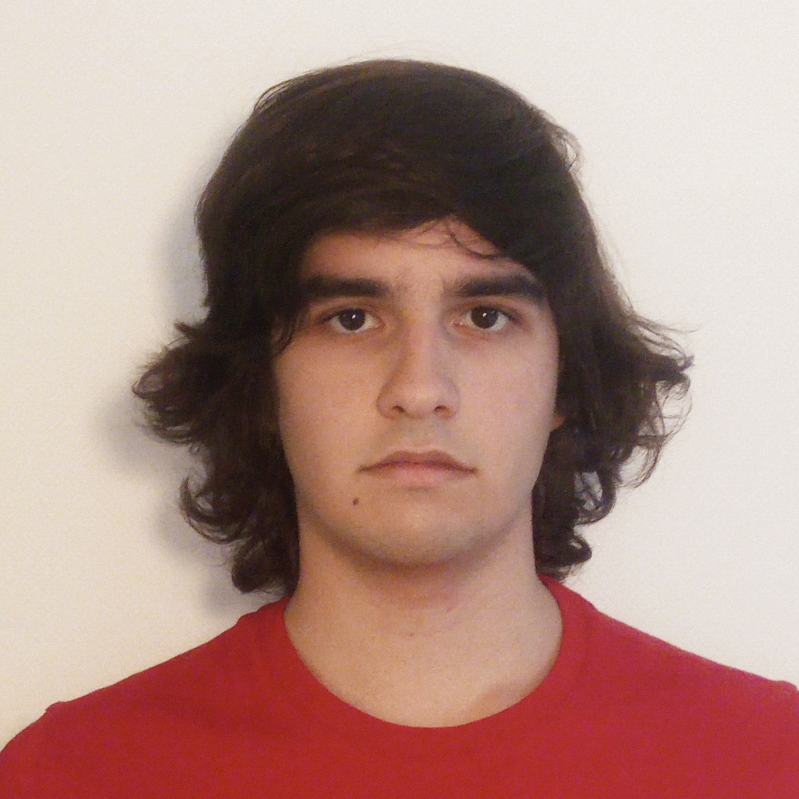
\includegraphics[width=3.5cm]{res/cover/A104348.png} \\

        Ana Oliveira & Humberto Gomes \\
        A104437      & A104348
    \end{tabular}

    \begin{tabular}{>{\centering}p{0.25\textwidth}
                    >{\centering\arraybackslash}p{0.25\textwidth}}
        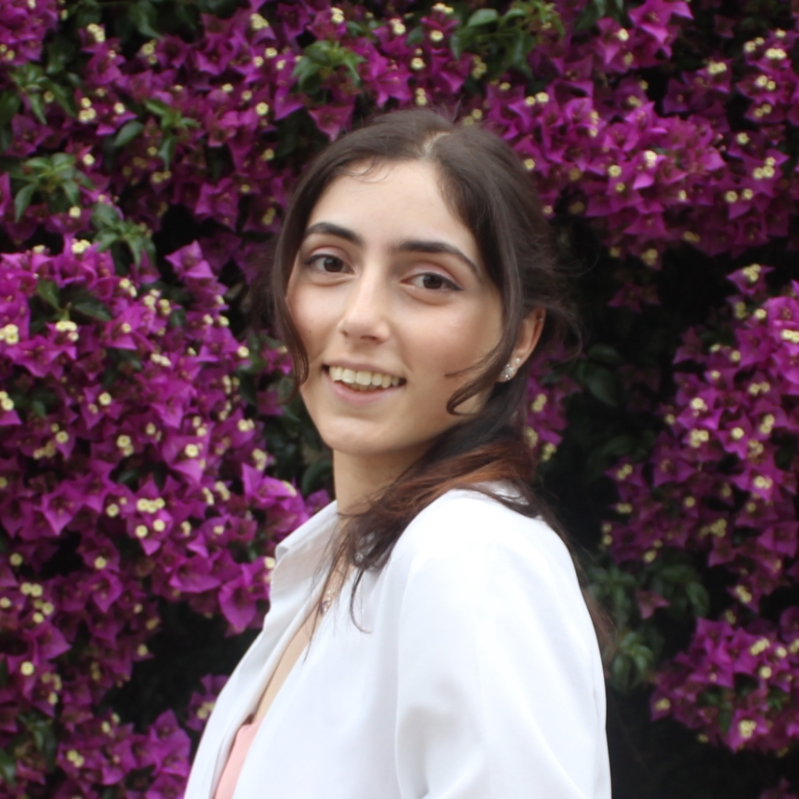
\includegraphics[width=3.5cm]{res/cover/A90817.png} &
        
\includegraphics[width=3.5cm]{res/cover/A104179.png} \\

        Mariana Cristino & Sara Lopes \\
        A90817           & A104179
    \end{tabular}
\end{center}

\begin{abstract}
    \textbf{\color{red} TODO - resumo}
\end{abstract}

\section{\emph{Generator}}

\textbf{\color{red} TODO - \emph{generator}}

\section{\emph{Engine}}

\textbf{\color{red} TODO - \emph{engine}}

\section{Resultados obtidos}

\textbf{\color{red} TODO - resultados}

\section{Conclusão e Trabalho Futuro}

\textbf{\color{red} TODO - conclusão}

% Isto é uma grande gambiarra, mas funciona para pôr a bibliografia como uma secção.
\section{Bibliografia}

\def\refname{}
\vspace{-1.5cm}
\begin{thebibliography}{9}
    \bibitem{exemplo}
        \href{https://youtu.be/dQw4w9WgXcQ}{Um item de exemplo na bibliografia}
\end{thebibliography}

\end{document}
